\section{Learning about Databases} 

\subsection{Por que?}

Las bases de datos toman un papel fundamental en el manejo de la informacion que se vive hoy en dia. En ellas es posible guardar datos de una manera estructurada, para luego poder consultarlos de una manera eficiente. Estas consultas pueden ser efectuadas en el orden de millones por segundo, y es necesario que la base de datos tenga resistencia ante tal caudal de procesamiento, y que sepa responder a cada consulta de una manera transparente.

Por este motivo en cualquier carrera de computacion o ingenieria de software se suele contar con un curso dedicado al entendimiento de estos motores. La profundidad con que se desarrolle el curso dependera del programa de cada carrera, pero es necesario contar con la mayor cantidad de herramientas posibles que permitan a cualquier interesado poder aprender cada uno de los aspectos que componen a un motor de base de datos.

Este paper introduce a Kanon, un motor de base de datos que provee una manera de conocer el funcionamiento de los administradores de transacciones, lockeo y recuperacion. Los mismos estan basados en los algoritmos de ARIES, por lo que se podra observar a un algoritmo de nivel industrial en funcionamiento. 

\begin{figure}[ht]
		\centering
		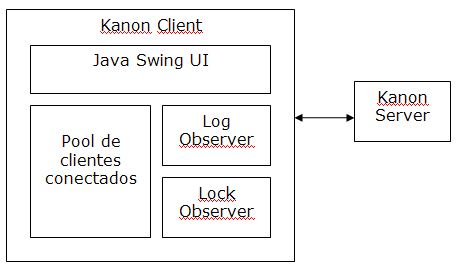
\includegraphics[scale=0.5]{img/arquitectura.png}
		\label{fig:arquitectura.png}
		\caption{Kanon Server Architecture}
\end{figure}

Este aporte le mostrar� al interesado c�mo se maneja el acceso a las tablas, de d�nde se obtienen los datos que satisfar�n las consultas requeridas, y c�mo es posible realizar modificaciones concurrentes a esas tablas sin temor a que se corrompan, y sabiendo que cualquier modificacion terminada nunca ser� perdida.

Con respecto a la concurrencia, el programa muestra la toma y liberacion de objetos de lockeo para acceder a cualquier registro, y cual es la varianza entre cada nivel de aislamiento. Se muestra como cada nivel cumple con lo que predica realizando distintos manejos a la hora de liberar los bloqueos tomado al escribir registros y como cada regla que uno encuentra en libros teoricos se cumple a la perfeccion manteniendo un orden parejo que no influye en las transacciones realizadas al motor. Por ejemplo, el nivel READ\_COMMITTED dicta que una transaccion no puede leer datos escritos por otra que no haya hecho commit. Para cumplir este requisito, antes que una transaccion escriba un dato, pide un lock exclusivo sobre el registro correspondiente. Si otra transaccion desea leer el valor de tal registro, primero debe pedir un lock de lectura. El administrador de lock fuerza que el pedido de la obtencion del lock de lectura se realice luego que el lock exclusivo sea liberado. Luego, el lock exclusivo de escritura se libera cuando la transaccion que lo obtuvo termina, ya sea por commit o por un rollback. Con esto el motor se asegura que las lecturas se hacen exclusivamente sobre datos escritos por transacciones terminadas. Este procedimiento puede ser comprobado por el usuario al ejecutar en Kanon dos consultas concurrentes sobre el mismo registro (la escritura primero) y observar en la tabla de lockeos como estos pedidos se ordenan y realizan de acuerdo al nivel READ\_COMMITTED.

El rollback es importante para garantizar la atomicidad de una transaccion. El motor muestra como cada operacion escribe en el log qu� fue lo que hizo, de manera tal de poder deshacer cada cambio en caso de que tenga que ser abortada. Tambien se muestra como las operaciones efectuadas durante el rollback se guardan tambien en el log, por si justo en ese momento el motor se cae y las operaciones deben repetirse la proxima vez que se levante, cuando se ejecute el administrador de recuperacion.



\begin{figure}[ht]
		\centering
		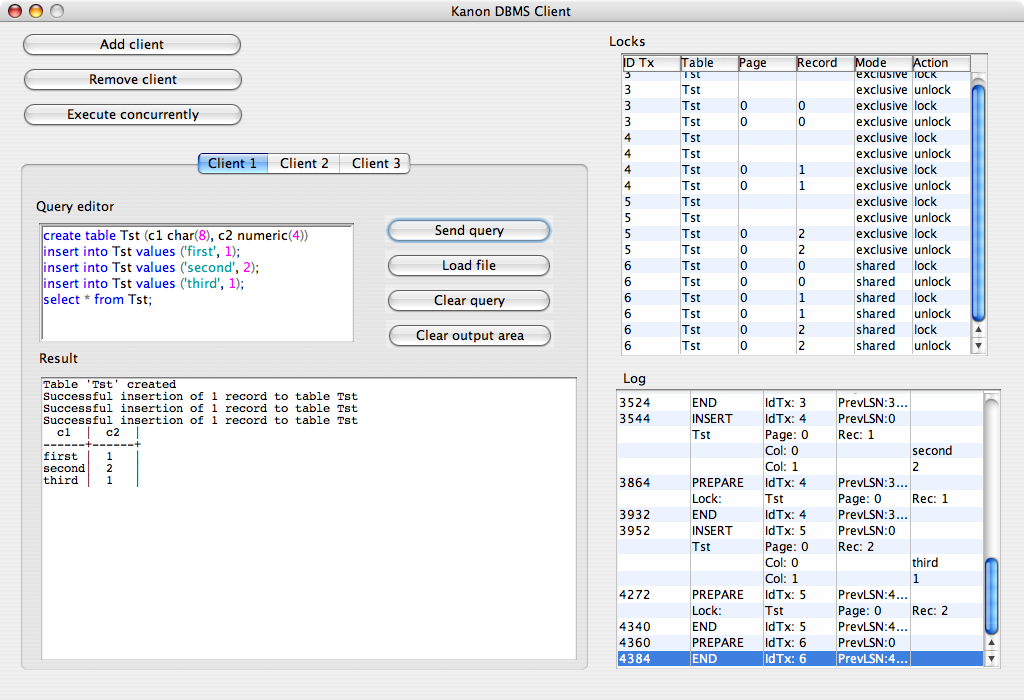
\includegraphics[scale=0.33]{img/KanonClienteMac.png}
		\label{fig:arquitectura.png}
		\caption{A client screenshot showing what how locks are acquired and released, and each operation gets saved into the log}
\end{figure}